\documentclass{article}
\usepackage{amsmath,amssymb,amsthm,latexsym,paralist,tikz}
\usetikzlibrary{arrows}

\theoremstyle{definition}
\newtheorem{problem}{P}
\newtheorem*{solution}{Solution}
\newtheorem*{resources}{Resources}

\newcommand{\name}[1]{\noindent\textbf{Name: #1}}
\newcommand{\honor}{\noindent On my honor, as an Aggie, I have neither
  given nor received any unauthorized aid on any portion of the
  academic work included in this assignment. Furthermore, I have
  disclosed all resources (people, books, web sites, etc.) that have
  been used to prepare this homework. \\[1ex]
 \textbf{Signature:} \underline{\hspace*{5cm}} }

 
\newcommand{\checklist}{\noindent\textbf{Checklist:}
\begin{compactitem}[$\Box$] 
\item Did you add your name? 
\item Did you disclose all resources that you have used? \\
(This includes all people, books, websites, etc. that you have consulted)
\item Did you sign that you followed the Aggie honor code? 
\item Did you solve all problems? 
\item Did you submit the pdf file resulting from your latex file 
  of your homework?
\item Did you submit a hardcopy of the pdf file in class? 
\end{compactitem}
}

\newcommand{\problemset}[1]{\begin{center}\textbf{Problem Set #1}\end{center}}
\newcommand{\duedate}[2]{\begin{quote}\textbf{Due dates:} Electronic
    submission of  this homework is due on \textbf{#1} on ecampus, a signed paper copy
    of the pdf file is due on \textbf{#2} at the beginning of
    class. \end{quote} }

\newcommand{\N}{\mathbf{N}}
\newcommand{\R}{\mathbf{R}}
\newcommand{\Z}{\mathbf{Z}}


\begin{document}
\problemset{7}
\duedate{3/20/2017 before 10:00am}{3/20/2017}
\name{Jonathan Janzen}
\begin{resources} Textbook, lecture slides, talking to classmates
\end{resources}
\honor

\newpage
\noindent\textbf{Problem 1 (BFS)}
\begin{problem} (15 points)
Exercise 22.2-5 on page 602. 
\end{problem}
\begin{solution}
Each element in the adjacency list that does not already have a value will be assigned the same value. Given some $u$ with $u.d = x$ in the graph, each element given by the adjacency list $v \in G.Adj[u]$ that has the value $v.d = \infty$ will be assigned the value $x+1$. Thus, vertexes that have already been visited will retain their $d$ values, and vertexes that have not been visited will all be assigned the same value, independent of order.\\
 \\
The case shown in the diagram uses an ordering where $t$ precedes $x$ in the adjacency list of $w$. An alternate ordering where $x$ is visited before $t$ the vertexes $u$ and $y$ will become children of $x$, whereas in the example $u$ became a child of $t$ and $y$ was the only child of $x$.
\end{solution}

\begin{problem} (15 points)
Exercise 22.2-6 on page 602. 
\end{problem}
\begin{solution} Using the following graph:\\
$$
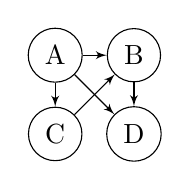
\begin{tikzpicture}
\tikzset{vertex/.style = {shape=circle,draw,minimum size=1.5em}}
\tikzset{edge/.style = {->,> = latex'}}
\node[vertex] (a) at  (0,1) {A};
\node[vertex] (b) at  (1,1) {B};
\node[vertex] (c) at  (0,0) {C};
\node[vertex] (d) at  (1,0) {D};

\draw[edge] (a) to (b);
\draw[edge] (a) to (c);
\draw[edge] (a) to (d);
\draw[edge] (b) to (d);
\draw[edge] (c) to (b);
\end{tikzpicture}
$$

And let $E_\pi = \{(A,C),(C,B),(B,D),(A,D),(A,B)\} \text{ and } s = A$\\
The shortest paths from the source vertex $A$ to any other vertex are all one edge long and given by the following:\\
$A \rightarrow B: (A,B)$\\
$A \rightarrow C: (A,C)$\\
$A \rightarrow D: (A,D)$\\
Which are all included in $E_\pi$. However, running BFS will use all the edges given by $E_\pi$ except for $(C,B)$ because that is a cross edge, and thus will be ignored by BFS. Therefore, this example demonstrates that all the simple paths from source to any other vertex (excluding the source vertex) in $E$ can be found using BFS on $E_\pi$, yet BFS will not utilize all edges in $E_\pi$.
\end{solution}

\begin{problem} (20 points)
(a) Exercise 22.2-8 on page 602. \\
(b) Prove that your algorithm returns the correct result. 
\end{problem}
\begin{solution}
Applying BFS from the source vertex $s$ we can check each vertex that BFS finds, denoted as $v$, we can check that node's $v.d$ property and compare it to some global variable $d$. If $v.d > d$ then $d$ becomes $v.d$ otherwise the value of $d$ does not change. This algorithm will run for each node in the tree (i.e. linear time, $O(V+E)$) and compare with $d$. At the end, the diameter of the tree will be $d$ because it will contain the greatest distance of any vertex from the source node $s$. The distance $d$ is defined as the diameter.
\end{solution}

\noindent\textbf{Problem 2 (DFS)}
\begin{problem} (15 points)
Exercise 22.3-5 on page 611.
\end{problem}
\begin{solution}
\textbf{a.} A forward edge indicates that the vertex $u$ precedes $v$ in a DFS. $u$ will therefore have a lesser $d$ value than $v$:
$$ u.d < v.d $$
A similar property holds for the finishing values, as DFS will finish vertexes in reverse order from when they were started, so $u$ will have a greater $f$ value than $v$:
$$ v.f < u.f $$
Finally, for any given vertex $x$, the $d$ value will be less than the $f$ value because the vertex must be found (indicated by $d$) before it is finished (indicated by $f$), so the following holds for $v$ and $u$:
$$ u.d < u.f \text{ and } v.d < v.f $$
Altogether, we can combine these into a single expression:
$$ u.d < v.d < v.f < u.f $$
Three of the inequalities are explicitly used, and the expression $u.d < u.f$ is implicitly used and can be found by deleting the middle terms ($v.d$, $v.f$)\\
\textbf{b.} A back edge is effectively the opposite of a forward edge (defined in part a). Therefore, given a vertex $u$ that precedes $v$ we have the following (borrowing from part a):
$$ v.d < u.d < u.f < v.f $$
This effectively swaps the vertexes used and mostly provides a definition. But there is one further constraint, an edge of the form ($v$, $v$) is also a back edge. Therefore, the inequality must allow $v=u$. In that case, $v.d = u.d$ and $v.f = u.f$, so the expression must be altered to include this possibility:
$$ v.d \leq u.d < u.f \leq v.f $$\\
\textbf{c.} For a cross edge, the vertexes $v$ and $u$ are not in the same subtrees, yet still have an edge connecting them. In a depth first search, one is visited and finished before the other. In this case let us assume that $v$ is visited before $u$, because the ordering of vertexes in adjacency lists is arbitrary and it cannot be known which vertex is visited first. In the case that $u$ is visited (and finished) first, the two can be swapped ($u$ becomes $v$ and $v$ becomes $u$). Thus, $v$ and $u$ are started before they are completed:
$$ v.d < v.f \text{ and } u.d < u.f $$
And since we are assuming that $v$ is visited first, we know that is completed before $u$ is started (DFS will go backtrack before iterating):
$$ v.f < u.d $$
Putting all this together, the final expression is:
$$ v.d < v.f < u.d < u.f $$
\end{solution}

\begin{problem} (15 points)
Exercise 22.3-8 on page 611.
\end{problem}
\begin{solution}
An example counterexample is provided below (double ended arrow indicating that a forward edge and back edge are both present):\\
$$
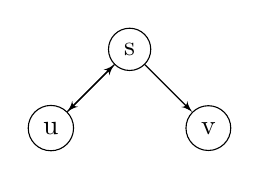
\begin{tikzpicture}
\tikzset{vertex/.style = {shape=circle,draw,minimum size=1.5em}}
\tikzset{edge/.style = {->,> = latex'}}
\node[vertex] (s) at  (1,1) {s};
\node[vertex] (u) at  (0,0) {u};
\node[vertex] (v) at  (2,0) {v};

\draw[edge] (s) to (u);
\draw[edge] (s) to (v);
\draw[edge] (u) to (s);
\end{tikzpicture}
$$
In this example, a path can be found from $u$ to $v$:
$$ \{(u,s),(s,v)\} $$
And given that $u.d < v.d$, we can see in this example that a DFS forest of the above tree the vertex $v$ would not be a descendent of $u$ because DFS will ignore the back edge $(u,s)$. Therefore, this is a counterexample due to the fact that $v$ is not a DFS descendant of $u$.
\end{solution}

\begin{problem} (20 points)
Prove that a directed graph $G$ has a cycle if and only if DFS($G$)
reveals a back edge. [You can use this property to make DFS-based
topological sorting robust against common user errors.] 
 \end{problem}
\begin{solution}
If there is a cycle, the forest given by DFS from any source vertex will have some number of forward edges that are part of the cycle and at least one back edge that completes the cycle. A back edge is defined as an edge that is found "out of order" with the other edges in that the timestamps for beginning and ending of the two nodes are reversed as compared to a forward edge (as shown in the definitions from problem 4 for a forward and back edge). The presence of a back edge indicates a way to go "backward" in the ordering and allow a cycle to occur. A primitive example can be found through some vertexes $v$ and $u$ where $u$ precedes $v$ in a DFS. A forward node from $u$ to $v$ is normal in a an acyclic graph and the constraint for a forward edge holds:
$$ u.d < v.d < v.f < u.f $$
However, consider the presence of an edge from $v$ to $u$ that allows the constraint for a back edge to hold:
$$ v.d \leq u.d < u.f \leq v.f $$
The presence of both a forward and a back edge in this case allows for a cycle, due to the fact that we can go back and forth from $u$ to $v$ while still following valid directed graph edges. This can be extended for cycles that contain more than two vertexes due to the fact that those examples could be simplified down to the point where they contain just one forward and back edge by deleting the middle vertexes reducing it to two vertexes with two edges between them. Now, the presence of only forward edges or only back edges would not introduce cycles, but the combination of one or more of each \textbf{does} produce cycles, and since back edges cannot occur without forward edges the presence of any back edge also indicates the presence of a forward edge.
\end{solution}



Discussions on ecampus are always encouraged, especially to clarify
concepts that were introduced in the lecture. However, discussions of
homework problems on piazza should not contain spoilers. It is okay to
ask for clarifications concerning homework questions if needed. 
\medskip



\goodbreak
\checklist
\end{document}
